\documentclass{article}
\usepackage[utf8]{inputenc}
\usepackage[margin=1.2in]{geometry}
\usepackage{hyperref}

\usepackage{tikz}
\usetikzlibrary{positioning}

\usepackage{natbib}
\usepackage{graphicx}
\usepackage{amsmath}
\usepackage{listings}
\usepackage{xcolor}


\definecolor{codegreen}{rgb}{0,0.6,0}
\definecolor{codegray}{rgb}{0.5,0.5,0.5}
\definecolor{codepurple}{rgb}{0.58,0,0.82}
\definecolor{backcolour}{rgb}{0.95,0.95,0.92}
\definecolor{deepblue}{rgb}{0,0,0.5}
\definecolor{deepred}{rgb}{0.6,0,0}
\definecolor{deepgreen}{rgb}{0,0.5,0}

\lstdefinestyle{mystyle}{
    backgroundcolor=\color{white},   
    commentstyle=\color{codegreen},
    keywordstyle=\color{deepblue},
    numberstyle=\tiny\color{codegray},
    stringstyle=\color{deepgreen},
    emph={Agent,__init__,act,self,union,exists, scope},
    emphstyle=\color{deepred},
    basicstyle=\ttfamily\footnotesize,
    breakatwhitespace=false,         
    breaklines=true,                 
    captionpos=b,                    
    keepspaces=true,                 
    numbers=left,                    
    numbersep=5pt,                  
    showspaces=false,                
    showstringspaces=false,
    showtabs=false,                  
    tabsize=3
}

\lstset{style=mystyle}

\title{\vspace{-2 cm}Universidade Federal de Ouro Preto \\ BCC 325 - Inteligência Artificial \\ Problemas de Satisfação de Restrições}
\author{Prof. Rodrigo Silva}
\date{}


\begin{document}

\maketitle

\section{Leitura}

\begin{itemize}
    \item Capítulo 3 do Livro\textit{ Artificial Intelligence: Foundations of Computational Agents,  2nd Edition} disponível em \textit{https://artint.info/}
    \item Capítulo 4 do Livro\textit{ Artificial Intelligence: Foundations of Computational Agents,  2nd Edition} disponível em \textit{https://artint.info/}
    \item Aquele que tudo sabe, tudo vê e nada teme.
\end{itemize}

\section{Questões}


\begin{enumerate}

%\item Considere o problema de encontrar um caminho no labirinto abaixo. O objetivo é ir da posição \textbf{s} até a posição \textbf{g}. O agente pode se mover horizontalmente e verticalmente. 
    
%\begin{enumerate}
    
%    \item No labirinto abaixo, numere os nós expandidos (visitados) por um agente que implementa o algoritmo de busca e profundidade. A ordem das ações é para cima, para a esquerda, para a direita, e para baixo. Assuma poda de ciclos.
%    \begin{figure}[!ht]
%        \centering
%        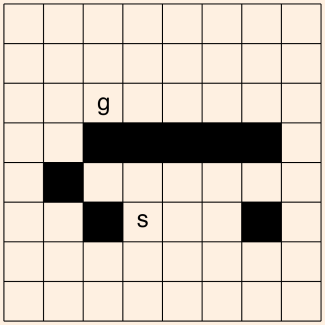
\includegraphics[width=0.7\textwidth]{grid.png}
%    \end{figure}
    
%\end{enumerate}

%\pagebreak
\subsection{Busca em espaços de estados}

\item  Preencha a seguinte tabela

    \begin{center}
        \begin{tabular}{|l|c|c|c|}
        \hline
        Estratégia            & Seleção da fronteira & Caminho Encontrado & Custo em Espaço \\
        \hline
        Busca em Largura      &     &   &   \\
        \hline
        Busca em Profundidade &     & (g)  &   \\
        \hline
        Guloso                &     &   &   \\
        \hline
        Menor Caminho Primeiro& (b) &   &   \\
        \hline
        $A^*$                 &     &   &   \\
        \hline
        Branch and Bound      &     &   &   \\
        \hline
    \end{tabular}
    \end{center}
    
    \begin{enumerate}
        \item Menor $h(n)$
        \item Menor $c(S,n)$
        \item Menor $h(n) + c(S,n)$
        \item Primeiro caminho adicionado 
        \item Último caminho adicionado 
        \item Menor número de arcos
        \item Indefinido
        \item Menor custo
        \item Linear 
        \item Exponencial
   
    \end{enumerate} 

\item Considere o código a seguir e responda.

\begin{figure}[!ht]
    \lstinputlisting[language=python]{agent.py}
    \caption{agent.py}
\end{figure}

\begin{enumerate}
    \item Que tipo de agente este código implementa?
    \item Qual parte do código corresponde a cada componente de um agente como definido no capítulo 2?
    \item Este agente fica preso em ciclos?
    \item Qual alteração devemos fazer para que o agente implemente uma poda de ciclos? Apresente o código da alteração. 
\end{enumerate}

\item O que é uma heurística admissível?

\subsection{Problemas de satisfação de restrições}

\item (Seção 4.1.3) Quais são os componentes de um problema de satisfação de restrições (Contraint Satisfaction Problem - CSP)? Apresente definições de cada componente.

\item Apresente aplicações reais que podem ser modeladas como problemas de satisfação de restrições?

\item Considere o problema a seguir:

\begin{align*}
    X &= \{A,B,C\} \\
    D &= \{\{1,2,3,4\},\{1,2,3,4\},\{1,2,3,4\} \}\\
    C &= \{ A >= B, B < C \}    
\end{align*}

\begin{enumerate}
    \item Qual o tamanho do espaço de busca? Ou seja, no pior caso, quantas soluções candidatas podem ser geradas?
    \item Apresente o pseudo-código de uma abordagem baseada em backtracking para resolver este problema.
    \item Apresente a árvore de chamadas do algoritmo backtracking para este problema.
    \item Represente este problema como uma rede de restrições?
\end{enumerate}

\item (Seção 4.4) Considere o Generalized Arc Concsistency (GAC) Algorithm apresentado abaixo e responda.

\begin{figure}[!t]
    \lstinputlisting[language=python]{pseudo_gac.py}
    \caption{Algoritmo GAC}
\end{figure}

\begin{enumerate}
    \item Demonstre a execução do algoritmo de consistência de arcos, GAC (Generalized Arc Consitency Algorithm) para o problema da questão anterior.
    \item Quais conclusões pode ser tiradas após a execução do GAC, no geral? O que podemos concluir após a execução do GAC para este problema?
    \item Após a execução do GAC, qual o tamanho do espaço de busca?
\end{enumerate}

\end{enumerate}

%\section{Projeto}

%\begin{enumerate}
%\item Nesta atividade você deve desenvolver um sistema agente/ambiente em que o agente explora um campo com obstáculos (ambiente). Dada um posição inicial e uma posição final, o agente deve encontrar o caminho de uma até a outra, desviando dos obstáculos, utilizando os seguinte algoritmos de busca:

%\begin{enumerate}
%    \item Busca em largura
%    \item Busca em profundidade
%    \item Algoritmo guloso
%    \item Menor custo primeiro
%    \item A*
%    \item Branch-and-bound
%\end{enumerate}

%\item  Preencha a seguinte tabela com experiência adquirida no projeto

%\begin{center}
%        \begin{tabular}{|l|c|c|c|}
%        \hline
%        Estratégia            & Seleção da fronteira & Caminho Encontrado & Custo em Espaço \\
%        \hline
%        Busca em Largura      &     &   &   \\
%        \hline
%        Busca em Profundidade &     & (g)  &   \\
%        \hline
%        Guloso                &     &   &   \\
%        \hline
%        Menor Caminho Primeiro& (b) &   &   \\
%        \hline
%        $A^*$                 &     &   &   \\
%        \hline
%        Branch and Bound      &     &   &   \\
%        \hline
%    \end{tabular}
%    \end{center}
    
%    \begin{enumerate}
%        \item Menor $h(n)$
%        \item Menor $c(S,n)$
%        \item Menor $h(n) + c(S,n)$
%        \item Primeiro caminho adicionado 
%        \item Último caminho adicionado 
%        \item Menor número de arcos
%        \item Indefinido
%        \item Menor custo
%        \item Linear 
%        \item Exponencial
%    \end{enumerate}
%\end{enumerate} 


   
% Na leitura recomendada você deve ter lido que agentes são entidades que interagem com um ambiente. Nesta atividade você deve implementar agentes que encontram o caminho de uma posição inicial até uma posição alvo desviando de objetos. 

% Visite o repositório \url{https://github.com/rcpsilva/BCC740\_ArtificialIntelligence}, que contem o código base para esta atividade e leia atentamente o README.

% O arquivo \textit{Room.py} contém a classe \texttt{Room} que implementa um \texttt{Environment} que representa uma sala com obstáculos. Atributos importantes desta classe são:

% \begin{itemize}
%     \item \texttt{room}: É uma matriz que contém 0 nas posições livres e 0 nas posições com obstáculos.
%     \item \texttt{initial\_positon}: Posição inicial do agente na sala.
%     \item \texttt{target}: Posição em que o agente deve chegar.
% \end{itemize}

% O método de classe \texttt{initial\_percepts()} retorna:

% \begin{itemize}
%     \item \texttt{current\_position}: com a posição inicial do agente.
%     \item \texttt{target}: com a posição em que o agente deve chegar.
%     \item \texttt{neighboors} com as posições vizinhas livres. 
% \end{itemize}

% O método de classe \texttt{signal(action)} retorna:

% \begin{itemize}
%     \item \texttt{current\_position}: com a posição atual do agente.
%     \item \texttt{target}: com a posição em que o agente deve chegar.(Obs: Esta opção está aqui para modelar a possibilidade de mudança de objetivo durante a execução.)
%     \item \texttt{neighboors} com as posições vizinhas livres. 
% \end{itemize}

% Uma \texttt{action} é, da lista de vizinhos livres, a posição para onde o agente quer se mover. 

% Veja o exemplo ilustrado na figura \ref{fig:room}.

% \begin{figure}[!ht]
%     \centering
%     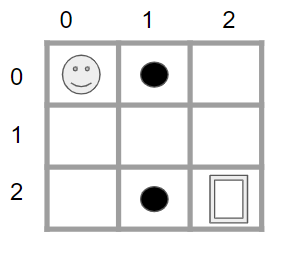
\includegraphics[width=0.4\textwidth]{room.PNG}
%     \caption{Ilustração da classe \texttt{Room}}
%     \label{fig:room}
% \end{figure}

% Para o exemplo mostrado na figura \ref{fig:room} teríamos:
%     \[
%         \texttt{room} = \begin{bmatrix}
%             0 & 1 & 0\\ 
%             0 & 0 & 0\\ 
%             0 & 1 & 0
%         \end{bmatrix}
%     \]
    
%     \[
%         \texttt{begin} = [0,0]
%     \]
    
%     \[
%         \texttt{target} = [2,2]
%     \]
    
%     \[
%         \texttt{current\_position} = [0,0]
%     \]
    
%     \[
%         \texttt{target} = [2,2]
%     \]
    
%     \[
%         \texttt{neighboors} = [[1,0],[1,1]]
%     \]

% o arquivo \textit{path\_finder\_agents.py} contém a implementação do \texttt{RandAgent}. Em cada posição, este agente escolhe um vizinho livre aleatoriamente para visitar. Ele para quando chega à posição alvo. Este agente pode ser usando como base para a implementação de outros agentes.

% Dadas estas informações, faça:

% \begin{enumerate}
%     \item Clone repositório \url{https://github.com/rcpsilva/BCC740\_ArtificialIntelligence}, leia atentamente o README e trabalhe a partir dele.
%     \item Execute o arquivo \textit{path\_finder\_simulation.py} para ver como o RandAgent se comporta.
%     \item No arquivo \textit{path\_finder\_agents.py}, implemente a classe \texttt{BFSAgent} que representa um agente que encontra a posição alvo fazendo uma busca em largura.
%     \item No arquivo \textit{path\_finder\_agents.py}, implemente a classe \texttt{DFSAgent} que representa um agente que encontra a posição alvo fazendo uma busca em profundidade.
%     \item No arquivo \textit{path\_finder\_agents.py}, implemente a classe \texttt{GreedyAgent} que representa um agente que encontra a posição alvo utilizando o algoritmo guloso.
%     \item No arquivo \textit{path\_finder\_agents.py}, implemente a classe \texttt{AStarAgent} que representa um agente que encontra a posição alvo utilizando o algoritmo A$^*$.
% \end{enumerate}

% Observações:
% \begin{itemize}
%     \item Todos os agentes implementados devem fazer poda de ciclos e poda de múltiplos caminhos.
%     \item Os agentes devem implementar a interface \texttt{Agent} definida no arquivo \textit{definitions.py}. 
%     \item Métodos auxiliares podem ser implementados para os agentes.
%     \item A classe $Room$ não deve ser modificada.
%     \item Os agentes implementados devem ser testados como indicado no arquivo \textit{path\_finder\_simulation.py}
% \end{itemize}
    

% %\bibliographystyle{plain}
% %\bibliography{references}
\end{document}

